\documentclass[11pt]{article}
\usepackage[a4paper,margin=2.2cm]{geometry}
\usepackage{amsmath,amssymb,mathtools,booktabs,array,xcolor,enumitem}
\usepackage{tikz}
\usetikzlibrary{quantikz,arrows.meta,positioning,calc}
\usepackage{url}
\usepackage[hidelinks,bookmarksnumbered]{hyperref}
\setlength{\parindent}{0pt}
\setlength{\parskip}{5pt}
\definecolor{fluxred}{HTML}{D62728}
\definecolor{boxblue}{HTML}{EAF2FB}
\definecolor{boxgreen}{HTML}{EDF7EA}
\definecolor{boxorange}{HTML}{FFF3E0}
\newcommand{\keyidea}[1]{\par\smallskip\noindent\fcolorbox{gray!60}{boxblue}{\begin{minipage}{\dimexpr\linewidth-2\fboxsep-2\fboxrule}\textbf{Key idea.} #1\end{minipage}}\par\smallskip}
\newcommand{\example}[2]{\par\smallskip\noindent\fcolorbox{gray!60}{boxgreen}{\begin{minipage}{\dimexpr\linewidth-2\fboxsep-2\fboxrule}\textbf{Example: #1.}\ #2\end{minipage}}\par\smallskip}
\newcommand{\numbers}[1]{\par\smallskip\noindent\fcolorbox{gray!60}{boxorange}{\begin{minipage}{\dimexpr\linewidth-2\fboxsep-2\fboxrule}\textbf{The numbers.} #1\end{minipage}}\par\smallskip}
\providecommand{\ket}[1]{|#1\rangle}
\providecommand{\bra}[1]{\langle #1|}
\newcommand{\CX}{\mathrm{CX}}
\newcommand{\Ry}{R_y}

\title{\textbf{How the plaq1 circuit was compressed}\\[4pt]
\large from 66\,468 to 202 two-qubit gates, explained step by step}
\author{su2qc-skqd project -- teaching note}
\date{28 October 2026}

\begin{document}
\maketitle

\begin{abstract}\noindent
This note explains, for a reader who knows basic linear algebra (vectors, matrices, the exponential of a
matrix) and has seen qubits before, how one piece of a quantum circuit -- the ``plaq1'' term of the
$2\times4$ SU(2) lattice gauge theory simulation -- was shrunk from 66\,468 two-qubit gates to 202, while
doing \emph{exactly} the same thing.  Every step is derived line by line and illustrated with the real
numbers and the real gates of the circuit.  All numbers were recomputed from the project's code (see
Section~\ref{sec:sources}); the compression itself was found by the genie-opus agent and checked
independently by a second agent.
\end{abstract}

\tableofcontents
\clearpage

%======================================================================
\section{The big picture}
%======================================================================

We simulate how a quantum system changes in time.  The quantum computer does this with a \emph{circuit}: a
list of operations (``gates'') on qubits.  The expensive gates are the \emph{two-qubit} gates, because on
real hardware each one has a small chance of error, and errors add up.  Fewer two-qubit gates means more
error-free runs.

One small piece of the full circuit is the \textbf{plaq1 term}: the magnetic energy of the middle square
(``plaquette'') of a ladder of $2\times4$ lattice sites.  In the original (``frozen'') circuit this one
piece alone needed 66\,468 two-qubit gates -- 93\% of the whole circuit.  The table shows where the
compression went; each line is a section of this note.

\begin{center}\small
\begin{tabular}{c l r c}
\toprule
step & idea & two-qubit gates & largest error\\
\midrule
0 & the original general-purpose method (Sec.~\ref{sec:step0}) & 66\,468 & $4.1\times10^{-13}$\\
1--3 & corner frames, a CNOT ladder, one rotation (Secs.~\ref{sec:step1}--\ref{sec:step3}) & 2\,110 & $3.4\times10^{-14}$\\
4 & spare qubits and ``dark'' flags (Sec.~\ref{sec:step4}) & 238 & $1.2\times10^{-14}$\\
5 & fewer rotation terms, chosen by a linear programme (Sec.~\ref{sec:step5}) & 220 & $9.5\times10^{-15}$\\
6 & the exact minimum, chosen by an integer programme (Sec.~\ref{sec:step6}) & 202 & $7.2\times10^{-15}$\\
\bottomrule
\end{tabular}
\end{center}

``Largest error'' compares each version with the exact mathematical operation on all 1\,831 allowed input
states; the project requires it to be below $10^{-10}$.  All versions pass by a wide margin, so the
compression changes the \emph{cost}, never the \emph{result}.

%======================================================================
\section{A toolkit of five facts}\label{sec:toolkit}
%======================================================================

Everything later is built from the five facts in this section.  It is worth reading slowly.

\subsection{Qubits, bit strings and the gates we use}

A qubit has two basis states $\ket0$ and $\ket1$.  Several qubits have basis states written as bit strings,
e.g.\ $\ket{101}$.  A general state is a weighted sum (a ``superposition'') of bit strings, with complex
weights called \emph{amplitudes}.  The gates we need:

\begin{center}
\renewcommand{\arraystretch}{1.25}
\begin{tabular}{l l l}
\toprule
gate & what it does & matrix\\
\midrule
$X$ (bit flip) & $\ket0\leftrightarrow\ket1$ & $\begin{pmatrix}0&1\\1&0\end{pmatrix}$\\
$\Ry(\phi)$ (rotation) & turns the state vector by the angle $\phi/2$ & $\begin{pmatrix}\cos\frac\phi2&-\sin\frac\phi2\\ \sin\frac\phi2&\cos\frac\phi2\end{pmatrix}$\\
CNOT, $\CX(c\to t)$ & flips $t$ if $c=1$ & $\ket{c,t}\mapsto\ket{c,\,t\oplus c}$\\
CZ & multiplies $\ket{11}$ by $-1$ & $\mathrm{diag}(1,1,1,-1)$\\
CP$(\lambda)$ & multiplies $\ket{11}$ by $e^{i\lambda}$ & $\mathrm{diag}(1,1,1,e^{i\lambda})$\\
\bottomrule
\end{tabular}
\end{center}
Here $\oplus$ is addition modulo 2 (``XOR''): $0\oplus0=0$, $0\oplus1=1\oplus0=1$, $1\oplus1=0$.
CNOT, CZ and CP are the two-qubit gates; they are the ones we count.

\subsection{Fact 1: the exponential of a bit flip is a rotation}

Our circuits must apply $e^{-i\theta h}$ for a Hamiltonian term $h$.  The simplest case is a term that flips
one qubit with strength $\sigma$: $h=\sigma X$.  Use the power series of the exponential and the fact
$X^2=I$ (flipping twice does nothing):
\begin{align*}
e^{-i\theta\sigma X}
&= \sum_{k=0}^{\infty}\frac{(-i\theta\sigma)^k}{k!}X^k\\
&= \underbrace{\Big(1-\frac{(\theta\sigma)^2}{2!}+\frac{(\theta\sigma)^4}{4!}-\cdots\Big)}_{\text{even }k:\ X^k=I}I
   \;-\;i\underbrace{\Big(\theta\sigma-\frac{(\theta\sigma)^3}{3!}+\cdots\Big)}_{\text{odd }k:\ X^k=X}X\\
&= \cos(\theta\sigma)\,I-i\sin(\theta\sigma)\,X
 =\begin{pmatrix}\cos\theta\sigma & -i\sin\theta\sigma\\ -i\sin\theta\sigma & \cos\theta\sigma\end{pmatrix}.
\end{align*}
So $\ket0\to\cos(\theta\sigma)\ket0-i\sin(\theta\sigma)\ket1$: amplitude slowly ``leaks'' from $\ket0$ to
$\ket1$.  Up to two fixed one-qubit gates this is the rotation $\Ry(2\theta\sigma)$.  \textbf{One flip with
one strength = one rotation.}

\subsection{Fact 2: a block-diagonal term splits into independent pieces}

If the states can be sorted into groups (``blocks'') so that $h$ never connects two different groups, then
$h$ is block-diagonal and so is its exponential, because every power $h^k$ is block-diagonal:
\[
h=\begin{pmatrix}h_1&0\\0&h_2\end{pmatrix}
\;\Rightarrow\;
h^k=\begin{pmatrix}h_1^k&0\\0&h_2^k\end{pmatrix}
\;\Rightarrow\;
e^{-i\theta h}=\begin{pmatrix}e^{-i\theta h_1}&0\\0&e^{-i\theta h_2}\end{pmatrix}.
\]
Each block evolves on its own.  If every block is a \emph{pair} of states, every block is just Fact 1.

\subsection{Fact 3: a ``frame'' (change of basis) can be applied and undone}

Let $F$ be any reversible circuit.  Then $(FhF^{-1})^k = FhF^{-1}FhF^{-1}\cdots FhF^{-1}=Fh^kF^{-1}$ (the
inner $F^{-1}F$ cancel), so, summing the power series,
\[
e^{-i\theta FhF^{-1}} = F\,e^{-i\theta h}\,F^{-1}
\qquad\Longleftrightarrow\qquad
\boxed{\,e^{-i\theta h}=F^{-1}\,e^{-i\theta h'}\,F,\quad h'=FhF^{-1}.\,}
\]
\keyidea{If we can find a cheap circuit $F$ (a ``frame'') that makes $h'$ \emph{simple}, we build the simple
$e^{-i\theta h'}$ instead and sandwich it between $F$ and $F^{-1}$.  The total is exactly the original
operation.  This is the trick behind the whole compression.}

\subsection{Fact 4: a multiplexed rotation, and why it costs $2^m$}

A \emph{multiplexed rotation} turns one target qubit by an angle that depends on $m$ control qubits:
\[
\sum_{c}\ket c\!\bra c\otimes \Ry(\theta_c),\qquad c=\text{the bit string of the controls}.
\]
How to build it?  First a key identity: an $X$ before and after a $y$-rotation reverses its direction.
\[
X\,\Ry(\phi)\,X=\begin{pmatrix}0&1\\1&0\end{pmatrix}
\begin{pmatrix}\cos\frac\phi2&-\sin\frac\phi2\\ \sin\frac\phi2&\cos\frac\phi2\end{pmatrix}
\begin{pmatrix}0&1\\1&0\end{pmatrix}
=\begin{pmatrix}\cos\frac\phi2&\sin\frac\phi2\\ -\sin\frac\phi2&\cos\frac\phi2\end{pmatrix}=\Ry(-\phi).
\]
Now the case $m=1$:
\begin{center}
\begin{quantikz}
\lstick{control $c$} & \qw & \ctrl{1} & \qw & \ctrl{1} & \qw\\
\lstick{target} & \gate{\Ry(\alpha_0)} & \targ{} & \gate{\Ry(\alpha_1)} & \targ{} & \qw
\end{quantikz}
\end{center}
If $c=0$ the CNOTs do nothing: the target gets $\Ry(\alpha_1)\Ry(\alpha_0)=\Ry(\alpha_0+\alpha_1)$.
If $c=1$ the second rotation is sandwiched by $X$'s: $X\Ry(\alpha_1)X\,\Ry(\alpha_0)=\Ry(\alpha_0-\alpha_1)$.
So
\[
\theta_0=\alpha_0+\alpha_1,\quad \theta_1=\alpha_0-\alpha_1
\quad\Longrightarrow\quad
\alpha_0=\tfrac{\theta_0+\theta_1}{2},\ \ \alpha_1=\tfrac{\theta_0-\theta_1}{2}.
\]
With $m$ controls the same idea needs $2^m$ rotations and $2^m$ CNOTs (the ``Gray-code'' construction): each
rotation $\alpha_S$ belongs to a subset $S$ of the controls, and
\begin{equation}\label{eq:walsh}
\theta_c=\sum_{S}\alpha_S\,(-1)^{|S\cap c|}
\end{equation}
(the sign is $-1$ for every control in $S$ that is 1).  This is called a \emph{Walsh expansion}; we come back
to it in Section~\ref{sec:step5}.
\keyidea{A multiplexed rotation with $m$ controls costs $2^m$ CNOTs.  Each extra control doubles the price.
Reducing the number of controls -- and the number of separate multiplexed rotations -- is what the
compression is about.}

\subsection{Fact 5: CNOTs can move a bit flip from one qubit to another}

Two-qubit truth table of $\CX(a\to b)$, then flip both qubits, then $\CX(a\to b)$ again:
\begin{center}
\begin{tabular}{c c c c}
\toprule
start $(a,b)$ & after $\CX$ & after flipping both & after $\CX$\\
\midrule
$(0,0)$ & $(0,0)$ & $(1,1)$ & $(1,0)$\\
$(0,1)$ & $(0,1)$ & $(1,0)$ & $(1,1)$\\
$(1,0)$ & $(1,1)$ & $(0,0)$ & $(0,0)$\\
$(1,1)$ & $(1,0)$ & $(0,1)$ & $(0,1)$\\
\bottomrule
\end{tabular}
\end{center}
In every row the net effect is: $a$ flipped, $b$ unchanged.  In operator language
$\CX\,(X_a X_b)\,\CX = X_a$.  The reason: after the first CNOT, $b$ holds $a\oplus b$, and flipping both $a$
and $b$ leaves $a\oplus b$ unchanged.  \textbf{A CNOT turns ``flip two qubits together'' into ``flip one''.}

%======================================================================
\section{The problem: what the plaq1 term does}\label{sec:problem}
%======================================================================

\subsection{The square and its 16 qubits}

\begin{center}
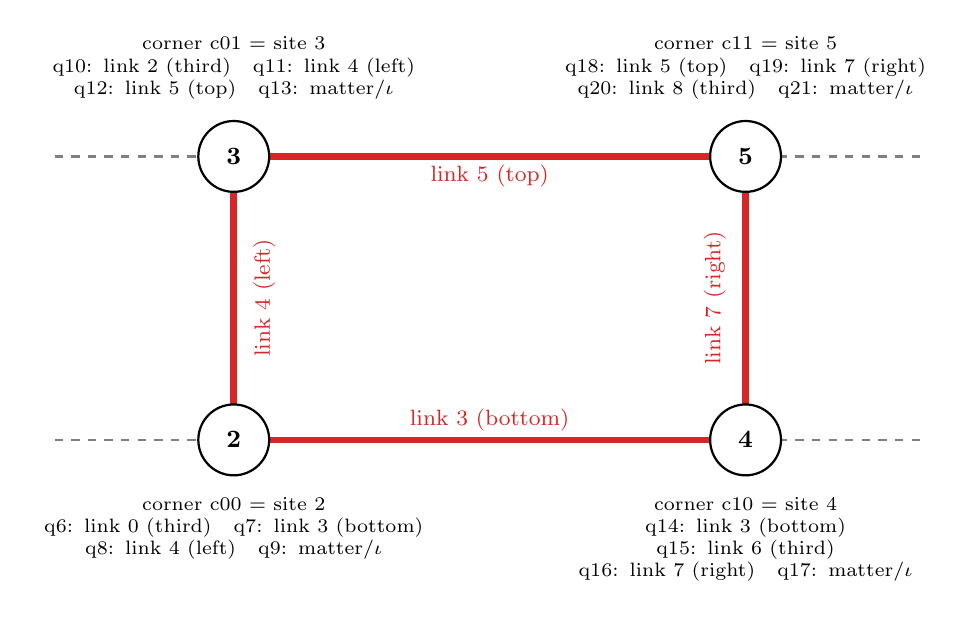
\begin{tikzpicture}[x=6.5cm,y=3.6cm,
  site/.style={circle,draw,thick,minimum size=0.9cm,font=\small\bfseries,fill=white},
  lab/.style={font=\scriptsize,align=center,text width=5.0cm}]
\draw[fluxred,line width=2.4pt] (0,0)--(1,0)--(1,1)--(0,1)--cycle;
\draw[gray,dashed,thick] (-0.35,0)--(0,0); \draw[gray,dashed,thick] (-0.35,1)--(0,1);
\draw[gray,dashed,thick] (1,0)--(1.35,0); \draw[gray,dashed,thick] (1,1)--(1.35,1);
\node[site] (a) at (0,0) {2}; \node[site] (b) at (1,0) {4}; \node[site] (c) at (1,1) {5}; \node[site] (d) at (0,1) {3};
\node[lab,below=4pt of a] {corner c00 = site 2\\q6: link 0 (third)\quad q7: link 3 (bottom)\\q8: link 4 (left)\quad q9: matter/$\iota$};
\node[lab,below=4pt of b] {corner c10 = site 4\\q14: link 3 (bottom)\quad q15: link 6 (third)\\q16: link 7 (right)\quad q17: matter/$\iota$};
\node[lab,above=4pt of c] {corner c11 = site 5\\q18: link 5 (top)\quad q19: link 7 (right)\\q20: link 8 (third)\quad q21: matter/$\iota$};
\node[lab,above=4pt of d] {corner c01 = site 3\\q10: link 2 (third)\quad q11: link 4 (left)\\q12: link 5 (top)\quad q13: matter/$\iota$};
\node[font=\footnotesize,text=fluxred] at (0.5,0.07) {link 3 (bottom)};
\node[font=\footnotesize,text=fluxred] at (0.5,0.93) {link 5 (top)};
\node[font=\footnotesize,text=fluxred,rotate=90] at (0.06,0.5) {link 4 (left)};
\node[font=\footnotesize,text=fluxred,rotate=90] at (0.94,0.5) {link 7 (right)};
\end{tikzpicture}
\end{center}

Each of the four corner sites owns four qubits (16 in total, q6--q21):
\begin{itemize}[itemsep=1pt]
\item three \textbf{flux bits}, one per link meeting at that site.  A flux bit is 1 if the link carries a unit
of colour-electric flux (spin $j=\tfrac12$), 0 if not ($j=0$).  Two of the links are sides of the square; the
third (dashed) leaves the square;
\item one \textbf{matter bit}: it stores how many quarks sit on the site, or -- when all three links carry
flux and there is one quark -- which of two possible spin arrangements, $\iota=0$ or $1$, the site is in.
\end{itemize}
Every link is stored \emph{twice}, once at each of its two end sites (e.g.\ link 3 is q7 and q14).  In a
physical state the two copies are always equal.

\subsection{What the term does}

The plaquette operator lays a closed loop of flux around the square or removes it.  It therefore flips all
four sides at once -- \emph{eight} qubits, because of the double storage:
\[
\text{q7, q14 (bottom)},\quad \text{q16, q19 (right)},\quad \text{q12, q18 (top)},\quad \text{q8, q11 (left)}.
\]
The \emph{strength} of the flip depends on the state of the corners (third links, quarks, $\iota$).  Some
states are not changed at all.

\numbers{Gauss's law (the rule that at every site the colour spins must cancel) allows only 13 of the 16
bit patterns of an interior site.  Combining four corners and requiring that the two copies of every side
agree leaves \textbf{1\,831 valid states} of the 16 qubits.  The term never mixes two states unless one can
be reached from the other by adding or removing the loop, so the 1\,831 states fall into \textbf{811
blocks} (Fact 2):}

\begin{center}
\begin{tabular}{l c c c c c c}
\toprule
block size & 1 & 2 & 3 & 4 & 5 & 9\\
number of blocks & 163 & 375 & 225 & 9 & 36 & 3\\
\bottomrule
\end{tabular}
\end{center}

\example{a block of size 2}{The empty square (no flux anywhere, all matter bits 0) and the square with one
flux loop around it form a pair.  The coupling between them is $\sigma=0.25$.  At the first time step of the
$B=0$ simulation the angle is $\theta=0.11470$, so by Fact 1 one step does
\begin{align*}
\ket{\text{empty}}\ \to\ &\cos(0.25\cdot0.11470)\ket{\text{empty}}-i\sin(0.25\cdot0.11470)\ket{\text{loop}}\\
=\ &0.99959\,\ket{\text{empty}}-0.02867\,i\,\ket{\text{loop}}.
\end{align*}
A small amount of amplitude moves into ``loop present''.}

\example{a block of size 3}{At corner c00, the state with flux only on the third link and one quark
(site bits q6\,q7\,q8\,q9 $=1000$) is connected to \emph{two} states: three flux links with $\iota=0$
(1110) and with $\iota=1$ (1111).  This one-to-two connection is the real difficulty; Section~\ref{sec:step1}
shows how it is removed.}

%======================================================================
\section{Step 0: the original method and why it cost 66\,468}\label{sec:step0}
%======================================================================

The package's general method (\texttt{circuits\_ir.structured\_term\_gates}) treats each block separately:
\begin{enumerate}[itemsep=1pt]
\item In each block it writes $e^{-i\theta h_{\rm block}}$ as a few \emph{rounds} of two-state rotations
(Fact 1 applied to pairs of basis states, after rotating the block into a convenient basis).
\item It merges into one multiplexed rotation (Fact 4) all rotations that are in the \textbf{same round} and
flip the \textbf{same set of qubits}.
\end{enumerate}

\numbers{Blocks of size 2 need 1 round; size 3 and 4 need 3; size 5 needs 13; size 9 needs 57.  (A
basis change among $n$ states takes up to $n(n-1)/2$ two-state rotations: $4\cdot3/2=6$ and
$8\cdot7/2=28$, so $6+1+6=13$ and $28+1+28=57$.)  Over the 57 rounds there are 82 different (round, flip
pattern) combinations, hence \textbf{82 multiplexed rotations}, with 7 to 11 controls each.}

The cost follows from Fact 4.  The controls histogram is
$\{7\!:\!1,\ 8\!:\!23,\ 9\!:\!29,\ 10\!:\!14,\ 11\!:\!15\}$, so the Gray-code cores cost
\begin{align*}
\sum 2^m &= 1\cdot2^7+23\cdot2^8+29\cdot2^9+14\cdot2^{10}+15\cdot2^{11}\\
&=128+5\,888+14\,848+14\,336+30\,720\\
&=65\,920\ \text{CNOTs (and the same number of } \Ry\text{)}.
\end{align*}
On top come 396 CNOTs that reduce controls and 152 CNOTs that squeeze each multi-bit flip onto one target
(Fact 5): $65\,920+396+152=\mathbf{66\,468}$.

\keyidea{Only 4 of the 82 multiplexed rotations actually move the flux loop.  The other 78 just rotate
between $\iota$ states, block by block.  The last 44 of them serve only the three size-9 blocks -- 132 small
rotations -- yet cost 25\,216 CNOTs.  The method is exact but blind to the structure of the problem.}

%======================================================================
\section{The key discovery: the plaquette is a product over corners}\label{sec:discovery}
%======================================================================

genie-opus tested whether the $1\,831\times1\,831$ matrix $h$ of the term can be written as a product of four
small $4$-qubit matrices, one per corner:
\[
h\big|_{\text{valid states}} = A_{c00}\otimes A_{c10}\otimes A_{c11}\otimes A_{c01}.
\]
It can, exactly: on every one of the 1\,831 rows the difference is at most $1.6\times10^{-15}$ (rounding
error).  Physically: the plaquette is a product of four link operators whose colour indices are tied
together at the corners, and gauge invariance makes each corner piece depend only on that corner.

\numbers{Each corner piece contains only a few different numbers.  For corner c00 (site 2):
\begin{center}\small
\begin{tabular}{l p{6.2cm} l}
\toprule
connection (q6\,q7\,q8\,q9) & what changes & strength\\
\midrule
$0000\leftrightarrow0110$ & empty corner $\leftrightarrow$ flux on both square sides & 0.74139\\
$0010\leftrightarrow0100$ & flux moves from one square side to the other & 0.52424\\
$1000\leftrightarrow\{1110,1111\}$ & three-state block (one flux $\to$ three flux, $\iota=0,1$) & 0.74139 (and 0)\\
\bottomrule
\end{tabular}
\end{center}
The two strengths are always in the ratio $0.52424/0.74139=0.70711=1/\sqrt2$, at every corner (corner c11:
$0.43380/0.61348=1/\sqrt2$).}

\example{the empty $\leftrightarrow$ loop coupling as a product}{All four corners go from ``no flux'' to
``flux on both square sides'':
\[
\sigma = 0.74139\times0.74139\times0.61348\times0.74139 = 0.2500,
\]
exactly the coupling 0.25 of the pair in Section~\ref{sec:problem}.}

\keyidea{Because the term is a product of four independent corner pieces, we can ``straighten'' each corner
separately with a few gates (Step 1), then join the corners (Step 2).}

%======================================================================
\section{Step 1: corner frames -- make each corner flip one qubit}\label{sec:step1}
%======================================================================

\subsection{1a. One CNOT per corner}

At corner c00 the plaquette flips q7 and q8 together.  By Fact 5, a CNOT q7$\to$q8 makes it flip only q7:
\[
\CX(7\to8)\,\big(X_7X_8\big)\,\CX(7\to8)=X_7 .
\]
After the CNOT, q8 holds $x=\text{q7}\oplus\text{q8}$: 0 if the two square sides at this corner agree, 1 if
they differ.  The plaquette never changes $x$; it becomes a \emph{label} that only influences the strength.
We call q7 ``$p_a$'' (the qubit that still flips) and q8 ``$p_b$''.  The same is done at the other corners:
$\CX(14\to16)$, $\CX(18\to19)$, $\CX(11\to12)$.

\subsection{1b. The bright rotation: one partner instead of two}

The three-state block $1000\leftrightarrow\{1110,1111\}$ is the problem: one state is connected to two.  The
plaquette applied to $\ket{1000}$ gives (computed from the package's matrix, identical in all 147 cases):
\[
O\ket{1000}\ \propto\ \tfrac12\ket{1110}_{\iota=0}-\tfrac{\sqrt3}{2}\ket{1111}_{\iota=1}.
\]
\emph{Why these numbers.}  Before the move, the third-link flux and the quark form a spin-0 pair.  The
plaquette creates the two new half-spins on the square sides as a spin-0 pair of their own.  The package,
however, labels states by pairing the spins differently ($\iota$ = total spin of third link + bottom link).
Rewriting ``(third, quark) paired, (bottom, left) paired'' in the other pairing is a standard SU(2) result
with weights $\sqrt{2J+1}/2$: $\tfrac12$ for $J=0$ and $\tfrac{\sqrt3}2$ for $J=1$.

Define the \textbf{bright} and \textbf{dark} combinations:
\[
\ket\beta=\tfrac12\ket{\iota{=}0}-\tfrac{\sqrt3}{2}\ket{\iota{=}1},\qquad
\ket\delta=\tfrac{\sqrt3}{2}\ket{\iota{=}0}+\tfrac12\ket{\iota{=}1}.
\]
Check that they are perpendicular: $\langle\delta|\beta\rangle=\tfrac{\sqrt3}2\cdot\tfrac12+\tfrac12\cdot(-\tfrac{\sqrt3}2)=0$.
So the plaquette connects $\ket{1000}$ \emph{only} to $\ket\beta$; $\ket\delta$ is never reached.  The three-state
block is really one pair plus one untouched state.

\begin{center}
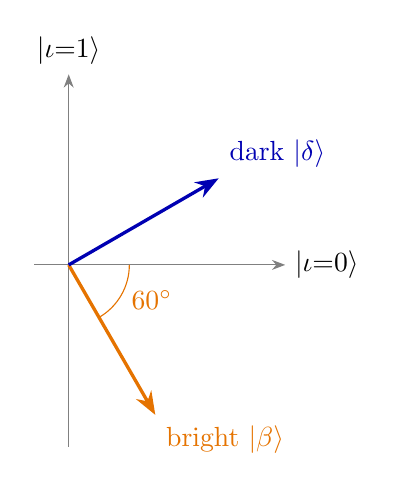
\begin{tikzpicture}[scale=2.2,>={Stealth}]
\draw[->,gray] (-0.2,0)--(1.25,0) node[right,black] {$\ket{\iota{=}0}$};
\draw[->,gray] (0,-1.05)--(0,1.1) node[above,black] {$\ket{\iota{=}1}$};
\draw[->,very thick,orange!90!black] (0,0)--(0.5,-0.866) node[below right] {bright $\ket\beta$};
\draw[->,very thick,blue!70!black] (0,0)--(0.866,0.5) node[above right] {dark $\ket\delta$};
\draw[orange!90!black] (0.35,0) arc[start angle=0,end angle=-60,radius=0.35];
\node[orange!90!black] at (0.48,-0.2) {$60^\circ$};
\end{tikzpicture}
\end{center}
The bright direction is $60^\circ$ below the $\ket{\iota{=}0}$ axis, because $\cos60^\circ=\tfrac12$ and
$\sin60^\circ=\tfrac{\sqrt3}2$.  Turning the $\iota$ qubit (q9) by $60^\circ$ puts the bright direction on one
axis and the dark direction on the other.  By the rotation formula a $60^\circ$ turn of the state is
$\Ry(120^\circ)$.  The code builds the rotation directly from the two computed overlaps $v_1,v_2$:
\[
R=\frac1{\sqrt{v_1^2+v_2^2}}\begin{pmatrix}v_1&v_2\\-v_2&v_1\end{pmatrix},\qquad
R\begin{pmatrix}v_1\\v_2\end{pmatrix}\!\frac{1}{|v|}=\begin{pmatrix}1\\0\end{pmatrix},\quad
R\begin{pmatrix}-v_2\\v_1\end{pmatrix}\!\frac{1}{|v|}=\begin{pmatrix}0\\1\end{pmatrix}.
\]
It must act \emph{only} when the corner is in the three-flux situation, so it is a multiplexed rotation on q9
with controls q6, q7, q8 (Fact 4, $m=3$, 8 CNOTs).  The real gates at corner c00:
\begin{center}
\resizebox{\linewidth}{!}{%
\begin{quantikz}[column sep=0.18cm,row sep=0.45cm]
\lstick{q6} & \qw & \qw & \qw & \ctrl{3} & \qw & \qw & \qw & \ctrl{3} & \qw & \qw & \qw & \ctrl{3} & \qw & \qw & \qw & \ctrl{3} & \qw & \qw & \qw & \qw\\
\lstick{q7} & \ctrl{1} & \qw & \qw & \qw & \qw & \ctrl{2} & \qw & \qw & \qw & \qw & \qw & \qw & \qw & \ctrl{2} & \qw & \qw & \qw & \qw & \qw & \qw\\
\lstick{q8} & \targ{} & \qw & \qw & \qw & \qw & \qw & \qw & \qw & \qw & \ctrl{1} & \qw & \qw & \qw & \qw & \qw & \qw & \qw & \ctrl{1} & \qw & \qw\\
\lstick{q9} & \qw & \gate{U} & \gate{+} & \targ{} & \gate{-} & \targ{} & \gate{+} & \targ{} & \gate{-} & \targ{} & \gate{-} & \targ{} & \gate{+} & \targ{} & \gate{-} & \targ{} & \gate{+} & \targ{} & \gate{U^\dagger} & \qw
\end{quantikz}}
\end{center}
(``$\pm$'' are $\Ry(\pm\pi/12)$; $U,U^\dagger$ are fixed one-qubit gates that align the rotation axis.)  We
checked by direct simulation: for the one control pattern (q6,\,q7,\,q8) $=(1,1,0)$ -- third link on, bottom
link on, sides agree, i.e.\ three flux links -- the eight pieces add up to $8\times\pi/12=120^\circ$; for the
other seven patterns they cancel to exactly $0^\circ$.

\example{what happens to the dark state}{Nothing.  After the rotation the dark combination sits on the basis
state $\ket{1111}$ and the plaquette's coupling to it is 0, so no gate touches it.  At the very end the
frame is undone and it returns to exactly the original combination of $\iota=0$ and $\iota=1$.  It is not
thrown away -- other terms of the Hamiltonian can still reach it.}

Corners c10 and c01 get the same pattern; corner c11 has no three-state block, so it gets only its CNOT.
After 1a and 1b every corner piece has the form ``flip $p_a$ $\times$ a number that depends on the corner's
labels''.

\subsection{1c. Fixing leftover signs}

After the frames, some of the corner numbers carry a minus sign that depends on the labels.  We remove each
with the cheapest gate that multiplies exactly the right states by $-1$:
\begin{itemize}[itemsep=1pt]
\item \textbf{free}: $\Ry(\phi+2\pi)=-\Ry(\phi)$, so adding $2\pi$ to a bright rotation flips a sign at no cost
(used at c00);
\item \textbf{CZ}: one two-qubit gate (used at c01, on q10 and q11);
\item \textbf{doubly-controlled Z (CCZ)}: multiplies $\ket{abc}$ by $(-1)^{abc}$ (used at c11).
\end{itemize}
How the CCZ is built from controlled phases.  A CP$(\lambda)$ gives the phase $e^{i\lambda\,uv}$ for bits $u,v$.
Using $a\oplus b=a+b-2ab$:
\begin{align*}
\tfrac\pi2\big[\,bc-(a\oplus b)c+ac\,\big]
&=\tfrac\pi2\big[\,bc-(a+b-2ab)c+ac\,\big]\\
&=\tfrac\pi2\big[\,bc-ac-bc+2abc+ac\,\big]=\pi\,abc ,
\end{align*}
and $e^{i\pi abc}=(-1)^{abc}$.  The real gates at c11 ($a$=q18, $b$=NOT q19, $c$=q20):
\begin{center}
\begin{quantikz}[column sep=0.3cm]
\lstick{q18} & \qw & \qw & \ctrl{1} & \qw & \ctrl{1} & \ctrl{2} & \qw & \qw\\
\lstick{q19} & \gate{X} & \ctrl{1} & \targ{} & \ctrl{1} & \targ{} & \qw & \gate{X} & \qw\\
\lstick{q20} & \qw & \gate{P(\frac\pi2)} & \qw & \gate{P(-\frac\pi2)} & \qw & \gate{P(\frac\pi2)} & \qw & \qw
\end{quantikz}
\end{center}
The first CP gives $\tfrac\pi2 bc$; the CNOT makes q19 hold $a\oplus b$, so the second CP gives
$-\tfrac\pi2(a\oplus b)c$; the next CNOT restores $b$; the last CP gives $\tfrac\pi2 ac$.  Cost: 3 CP + 2 CX = 5
two-qubit gates.

%======================================================================
\section{Step 2: the CNOT ladder -- one flip for the whole square}\label{sec:step2}
%======================================================================

After Step 1 the plaquette flips four qubits together: q7, q14, q18, q11 (one per corner).  Apply Fact 5
three times, all from q7:
\begin{center}
\begin{quantikz}[column sep=0.4cm]
\lstick{q7} & \ctrl{1} & \ctrl{2} & \ctrl{3} & \qw\\
\lstick{q14} & \targ{} & \qw & \qw & \qw\\
\lstick{q18} & \qw & \targ{} & \qw & \qw\\
\lstick{q11} & \qw & \qw & \targ{} & \qw
\end{quantikz}
\qquad
$L\,(X_7X_{14}X_{18}X_{11})\,L^{-1}=X_7$.
\end{center}
Line by line, with original values $a,b,c,d$:
\begin{center}
\begin{tabular}{l c c c c}
\toprule
stage & q7 & q14 & q18 & q11\\
\midrule
original & $a$ & $b$ & $c$ & $d$\\
after the ladder & $a$ & $b\oplus a$ & $c\oplus a$ & $d\oplus a$\\
plaquette flips all four & $\bar a$ & $\bar b\oplus\bar a=b\oplus a$ & $c\oplus a$ & $d\oplus a$\\
after undoing the ladder & $\bar a$ & $(b\oplus a)\oplus\bar a=\bar b$ & $\bar c$ & $\bar d$\\
\bottomrule
\end{tabular}
\end{center}
($\bar a$ = flipped $a$.)  In the ladder's labels only q7 changes; when the ladder is undone the flip is handed
back to the other three.  This also works for superpositions, because every step is linear.

\keyidea{The other three qubits \emph{do} flip -- the ladder just stores them relative to q7 so that, in the
middle of the circuit, a single qubit carries the whole flip.  Any of the four could have been chosen;
the code simply takes the first corner's $p_a$, q7.}

%======================================================================
\section{Step 3: one rotation does the whole term}\label{sec:step3}
%======================================================================

Let $F$ be Steps 1--2 together.  In the frame, the term has become (Fact 3)
\[
h'=FhF^{-1}=X_7\otimes \mathrm{diag}\big(F(s)\big),
\]
``flip q7, with a strength $F(s)$ that depends on the other 15 qubits $s$''.  Then, applying Fact 1 separately
for every value of $s$ (Fact 2: different $s$ never mix),
\[
e^{-i\theta h'}=\sum_s \ket s\!\bra s\otimes\Big(\cos\big(\theta F(s)\big)I-i\sin\big(\theta F(s)\big)X_7\Big),
\]
which is \textbf{one} multiplexed rotation on q7 (Fact 4).  The 1\,831 states now form 648 pairs that differ
only in q7 (each with its own angle) plus $1\,831-2\cdot648=535$ states with $F=0$ (left alone).

\numbers{The angle still depends on 11 of the other qubits, so the rotation costs $2^{11}=2\,048$ CNOTs.  The
frame costs $4$ (corner CNOTs) $+\,3\times8$ (bright rotations) $+\,3$ (ladder) $=31$, applied and undone:
\[
2\,048+2\times31=\mathbf{2\,110}\quad(\text{was }66\,468).
\]}
\keyidea{All 82 rotations collapsed into one, because after the frame every pair flips the \emph{same} qubit
in a \emph{single} round.  Steps 4--6 now make that one rotation cheaper.}

%======================================================================
\section{Step 4: spare qubits and dark-state flags}\label{sec:step4}
%======================================================================

Why 11 controls?  The strength depends on (i) whether the sides agree at each corner, $x_c$ (4 bits), and
(ii) whether each corner is on its dark state.  ``Dark'' is spread over two qubits per corner (third-link
bit \emph{and} matter bit both equal to 1), so (ii) needs up to 8 bits.

\subsection{4a. Free scratch qubits}

Because every side is stored twice, some qubits carry redundant information.  After the ladder, q14, q18,
q11 and q12 hold values that are fixed XOR-combinations of other qubits on \emph{every} valid state.

\example{a redundancy}{Each square side appears at two corners, so
\[
x_{c00}\oplus x_{c10}\oplus x_{c11}\oplus x_{c01}
=(\ell_3\oplus\ell_4)\oplus(\ell_3\oplus\ell_7)\oplus(\ell_5\oplus\ell_7)\oplus(\ell_4\oplus\ell_5)=0,
\]
($\ell$ = flux of a side), because every $\ell$ appears twice and $\ell\oplus\ell=0$.  So $x_{c01}$ is always
$x_{c00}\oplus x_{c10}\oplus x_{c11}$ and need not be stored separately.}

Applying CNOTs that XOR such a combination back into a qubit resets it to $\ket0$ on every valid state.  Six
CNOTs give \textbf{four clean qubits} (q14, q18, q11, q12).

\subsection{4b. One flag bit per corner}

Into each clean qubit we write $g_c=(\text{third-link bit})\ \mathrm{AND}\ (\text{matter bit})$, which is 1
exactly when corner $c$ is on its dark state.  The gate is a ``relative-phase Toffoli'' (3 CNOTs instead of
the 6 of a full Toffoli); it computes the AND up to a sign that cancels when the same gates are undone at the
end.  The real gates for corner c00 ($g$ = q6 AND q9, into q14):
\begin{center}
\begin{quantikz}[column sep=0.3cm]
\lstick{q6} & \qw & \qw & \qw & \ctrl{2} & \qw & \qw & \qw & \qw\\
\lstick{q9} & \qw & \ctrl{1} & \qw & \qw & \qw & \ctrl{1} & \qw & \qw\\
\lstick{q14} & \gate{\Ry(\frac\pi4)} & \targ{} & \gate{\Ry(\frac\pi4)} & \targ{} & \gate{\Ry(-\frac\pi4)} & \targ{} & \gate{\Ry(-\frac\pi4)} & \qw
\end{quantikz}
\end{center}

\subsection{4c. The angle now depends on 7 bits}

With the flags the strength becomes
\[
F(x,g)=\theta\,M(x)\prod_{c}\big(1-\bar x_c\,g_c\big),\qquad
|M(x)|=0.25\times\big(\tfrac1{\sqrt2}\big)^{\#\{c:\ x_c=1\}}.
\]
Read it as: start from 0.25; every corner whose sides disagree weakens it by $1/\sqrt2$; a dark corner whose
sides agree switches it off.  This needs the three independent $x$ bits (q8, q16, q19) and four flags (q14,
q18, q11, q12): \textbf{7 controls}, $2^7=128$ CNOTs.

\numbers{Frame per side $=4$ corner CNOTs $+\,3\times8$ bright $+\,1$ CZ $+\,5$ CCZ $+\,3$ ladder $+\,6$ clear
$+\,4\times3$ flags $=55$.  Total $128+2\times55=\mathbf{238}$ (was 2\,110).}

%======================================================================
\section{Step 5: fewer terms in the rotation (sparse Walsh)}\label{sec:step5}
%======================================================================

Recall Eq.~\eqref{eq:walsh}: the rotation is built from terms $\alpha_S$, one per subset $S$ of the controls;
each nonzero term costs a rotation and some CNOTs.  The standard (Gray-code) circuit uses all $2^m$ terms.
But some entries $\theta_c$ of the angle table are \textbf{free}: their control pattern $c$ never occurs on a
valid state, so we may give them any value.  Choosing them well can make many $\alpha_S$ zero.

\example{two controls, one free entry}{Suppose $\theta_{00}=\theta_{01}=\theta_{10}=t$ and $\theta_{11}=f$
is free.  Inverting Eq.~\eqref{eq:walsh} (multiply by the signs and average):
\[
\alpha_S=\tfrac14\sum_c\theta_c\,(-1)^{|S\cap c|}:\qquad
\begin{aligned}
\alpha_{00}&=\tfrac14(t+t+t+f)=\tfrac{3t+f}4,\\
\alpha_{01}&=\tfrac14(t-t+t-f)=\tfrac{t-f}4,\\
\alpha_{10}&=\tfrac14(t+t-t-f)=\tfrac{t-f}4,\\
\alpha_{11}&=\tfrac14(t-t-t+f)=\tfrac{f-t}4.
\end{aligned}
\]
With $f=0$ all four terms are nonzero (4 rotations).  With $f=t$ only $\alpha_{00}=t$ survives: \textbf{one}
rotation and no CNOTs.  Same action on every valid input, a quarter of the cost.}

For plaq1's rotation: 128 table entries, 120 fixed by physics, 8 free.  A linear programme (minimise
$\sum_S|\alpha_S|$, a smooth stand-in for ``number of nonzero terms'') chooses the free entries; then terms
are pruned and the rest re-solved exactly.

\numbers{103 terms used, visited in an order needing 110 CNOTs (Gray code: 128).  Total
$110+2\times55=\mathbf{220}$.}

%======================================================================
\section{Step 6: the exact minimum (integer programming)}\label{sec:step6}
%======================================================================

``Number of nonzero terms'' is not smooth, so the linear programme can only approximate it.  A
\emph{mixed-integer linear programme} (MILP) counts it exactly by adding a yes/no switch $z_S\in\{0,1\}$ per
term:
\[
\min\ \sum_S z_S\quad\text{subject to}\quad
\theta_c=\sum_S\alpha_S(-1)^{|S\cap c|}\ \ (\text{fixed }c),\qquad
-M z_S\le\alpha_S\le M z_S .
\]
If a switch is 0, its term is forced to 0; the solver (HiGHS) searches the switch settings by
\emph{branch and bound}, which also proves a lower bound.  In the two-control example above the MILP finds
$z=(1,0,0,0)$ with $f=t$: one term, proved optimal.

\numbers{For plaq1: 85 terms, 92 CNOTs.  After 1\,500 seconds the solver had proved that at least 78 terms are
needed in this construction, so at most 7 more could ever be saved this way.  Total $92+2\times55=\mathbf{202}$.
The same build makes every structural choice from angle-free tables, so the circuit has identical gates for
every time step $k$; only the angles change.}

%======================================================================
\section{Putting it together}\label{sec:together}
%======================================================================

\begin{center}
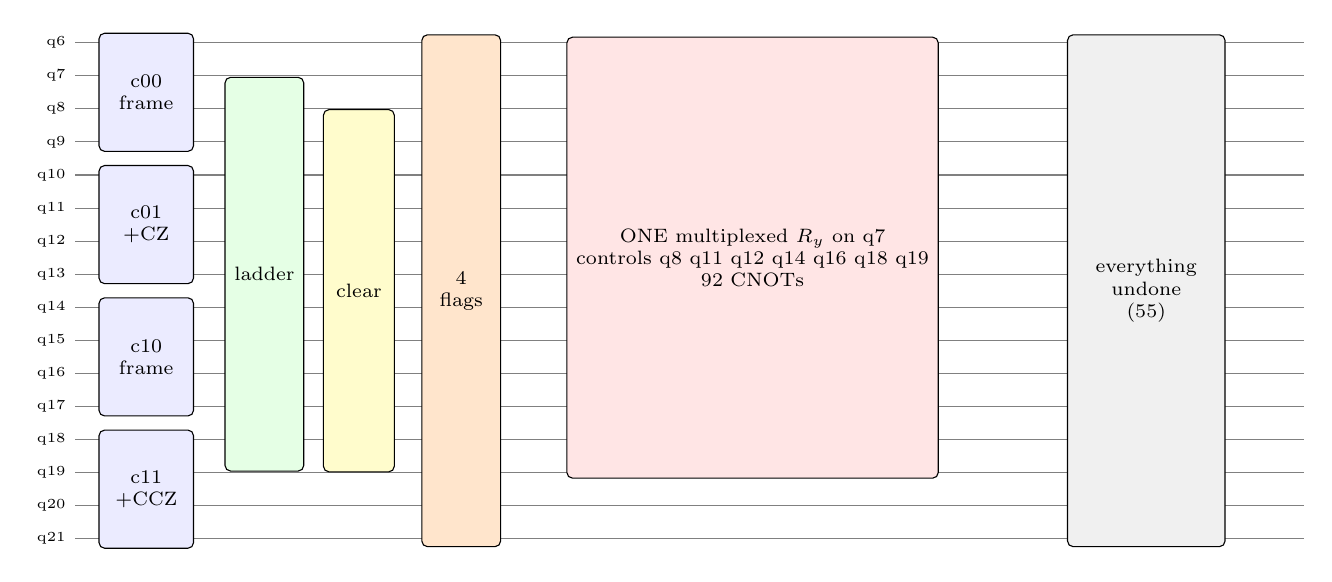
\begin{tikzpicture}[x=1cm,y=0.42cm,box/.style={draw,rounded corners=2pt,align=center,font=\scriptsize}]
\foreach \q [count=\i from 0] in {6,...,21} { \draw[gray] (0,-\i)--(15.6,-\i); \node[left,font=\tiny] at (0,-\i) {q\q}; }
\node[box,fill=blue!8,minimum height=1.5cm,minimum width=1.2cm] at (0.9,-1.5) {c00\\frame};
\node[box,fill=blue!8,minimum height=1.5cm,minimum width=1.2cm] at (0.9,-5.5) {c01\\+CZ};
\node[box,fill=blue!8,minimum height=1.5cm,minimum width=1.2cm] at (0.9,-9.5) {c10\\frame};
\node[box,fill=blue!8,minimum height=1.5cm,minimum width=1.2cm] at (0.9,-13.5) {c11\\+CCZ};
\node[box,fill=green!10,minimum height=5.0cm,minimum width=0.9cm] at (2.4,-7) {ladder};
\node[box,fill=yellow!20,minimum height=4.6cm,minimum width=0.9cm] at (3.6,-7.5) {clear};
\node[box,fill=orange!20,minimum height=6.5cm,minimum width=1.0cm] at (4.9,-7.5) {4\\flags};
\node[box,fill=red!10,minimum height=5.6cm,minimum width=4.6cm] at (8.6,-6.5) {ONE multiplexed $R_y$ on q7\\controls q8 q11 q12 q14 q16 q18 q19\\92 CNOTs};
\node[box,fill=gray!12,minimum height=6.5cm,minimum width=2.0cm] at (13.6,-7.5) {everything\\undone\\(55)};
\end{tikzpicture}
\end{center}

\begin{center}
\begin{tabular}{p{4.2cm} r p{7.6cm}}
\toprule
part & 2q gates & role\\
\midrule
frame $F$ (Steps 1, 2, 4a, 4b) & 55 & relabel so that only q7 flips, with a 7-bit-controlled strength\\
one rotation (Steps 3, 5, 6) & 92 & the actual physics: loop on/off, all 648 pairs at once\\
$F^{-1}$ & 55 & restore the original meaning of every qubit\\
\midrule
total & \textbf{202} & was 66\,468: $329\times$ fewer\\
\bottomrule
\end{tabular}
\end{center}

\paragraph{Why it is still exact.}  Every step is an exact identity (Facts 1--5), not an approximation.
Each version of the term was compared with the exact $e^{-i\theta h}$ on all 1\,831 valid states: largest
error $4.1\times10^{-13}$ (step 0), $3.4\times10^{-14}$, $1.2\times10^{-14}$, $9.5\times10^{-15}$ and
$7.2\times10^{-15}$ (step 6) -- rounding error only, far below the required $10^{-10}$.  The full 28-qubit
circuits containing the compressed term were checked again with an independent simulator.  The general
identities used here (frame conjugation, the ladder, the flip-times-diagonal exponential, the CCZ
construction, the relative-phase Toffoli cancellation, commuting Walsh terms) are proved in the Lean theorem
prover; the specific numbers of this term (its factorisation, signs and tables) are checked numerically.

\paragraph{What was really exploited.}
\begin{center}
\begin{tabular}{l l}
\toprule
step & structure of the physics that made it possible\\
\midrule
1--3 & the plaquette is a product over corners; SU(2) recoupling gives one bright partner\\
4 & links are stored twice (free scratch space); ``dark'' is a 1-bit condition\\
5--6 & angle-table entries for impossible inputs are free\\
\bottomrule
\end{tabular}
\end{center}

%======================================================================
\section{Where the numbers come from}\label{sec:sources}\sloppy
%======================================================================
\begin{itemize}[itemsep=1pt]
\item Frozen method: \path{validation/S2_2x4.json} (\path{data.synth['2x4|exact'].plaq1}: 66\,468 CX,
65\,920 $R_y$, 82 rotations, controls histogram, 198 frame CNOTs); blocks and states:
\path{data.structure.structure_4}.  The round-by-round breakdown was re-derived by re-running the package
builder.
\item Compression steps 1--6: rebuilt for these notes with genie-opus's code
(\path{2x4_compression_using_ai_v1/src/c2x4}: \path{plaqfactor.cf1_gates}, \path{cf2_gates},
\path{sparsemux}, \path{linsynth}), counted and verified against the exact term; equal to the stored
archive values in \path{data/archive_it1..6.json}.
\item Corner pieces: \path{data/p2_1_structure.json}.  MILP bound: \path{data/cert_it6_operator_plaq1_long.json}.
\item Bright/dark coefficients: read from the package's plaquette matrix (\path{skqd.reference_sim.localize}),
all 147 cases at corner c00.
\item Companion documents: \path{reports/plaq1_compression_steps_2x4.pdf} (circuit pictures),
\path{reports/valid_states_2x4_plaquettes.pdf} (every valid state of each plaquette),
\path{2x4_compression_using_ai_v1/reports/003-full-compression-report.md} (full technical report).
\end{itemize}

\appendix
\section{Glossary}
\begin{description}[itemsep=1pt,font=\normalfont\bfseries]
\item[Amplitude] complex weight of a bit string in a quantum state; its squared size is a probability.
\item[Block] a group of states that the term mixes only among themselves.
\item[Bright / dark state] the combination of the two $\iota$ states that the plaquette reaches / the one it never reaches.
\item[CNOT, CX] flips the target qubit if the control qubit is 1.
\item[Frame] a reversible circuit applied before and undone after an operation, to make it simpler (Fact 3).
\item[Flag] a qubit holding a computed yes/no fact (here: ``this corner is dark'').
\item[Gauss's law] at every site the colour spins must cancel; it decides which states are allowed.
\item[$\iota$ (intertwiner)] which of two ways four spin-$\tfrac12$ objects at a site cancel to spin 0.
\item[Multiplexed rotation] a rotation of one qubit whose angle depends on $m$ control qubits; costs $2^m$ CNOTs.
\item[Plaquette] one square of the lattice; its term adds or removes a loop of flux around it.
\item[Walsh expansion] writing the angle table of a multiplexed rotation as a sum of $\pm$ terms, Eq.~\eqref{eq:walsh}.
\item[XOR, $\oplus$] addition modulo 2.
\end{description}

\end{document}
